\chapter{Guía de usuario de la aplicación de control}\label{chap:appendixA}

\section{Instalación de los drivers y la aplicación}

Antes de poder utilizar la aplicación es preciso instalar correctamente en
el equipo la tarjeta de adquisición y los drivers de la tarjeta. Los
drivers pueden descargarse desde el sitio web del fabricante
(\url{http://www.keithley.com}).

Para poder utilizar la aplicación es necesario haber instalado previamente
en el \pc{} anfitrión una distribución de \matlab{} (revisión posterior a
2006a).

Para instalar la aplicación copiar el archivo \func{single\_channel.m} y el
archivo con extensión \func{single\_channel.fig} en el directorio de
trabajo.


\section{Especificaciones}

Para obtener información acerca de las prestaciones y limitaciones de la
aplicación véase el \vref{subsec:transducerconclusions}.


\section{Procedimientos de llamada}

Desde la ventana principal de \matlab{} es posible lanzar la aplicación de
tres modos diferentes.

\begin{itemize}
    \item En el navegador del sistema de archivos click derecho en el
	fichero \func{single\_channel.m}. Después seleccionar la opción
	<<ejecutar archivo>>.
    \item Ejecutar \sig{guide} (editor de interfaces gráficas de usuario).
	Abrir el fichero \func{single\_channel.fig}. Después click en el
	botón ejecutar de \sig{guide}.
    \item En el prompt de la ventana de comandos introducir el siguiente
	comando (cerciorarse previamente de que \matlab{} se encuentra en
	el directorio de trabajo).

	\begin{center}
	    \begin{lstlisting}[gobble=12]
		[handles = ]single_channel[(opciones)]
	    \end{lstlisting}
	\end{center}
\end{itemize}

El tercer procedimiento de llamada da acceso a las variables almacenadas en
el dominio interno de la aplicación como, por ejemplo: el búffer en el que se
almacenan las muestras recogidas o el objeto dispositivo que controla el
comportamiento de la tarjeta de adquisición.

La aplicación reutiliza cualquier objeto dispositivo asociado a la tarjeta
de adquisición, si no lo hubiera crea uno propio.


\section{Interfaz de usuario}

La \vref{fig:interface} muestra el aspecto de la interfaz gráfica de
usuario de la aplicación. La interfaz gráfica permite la interacción con el
sistema de medida, pueden encontrarse en ella 6 paneles.

\begin{figure}
    \begin{center}
	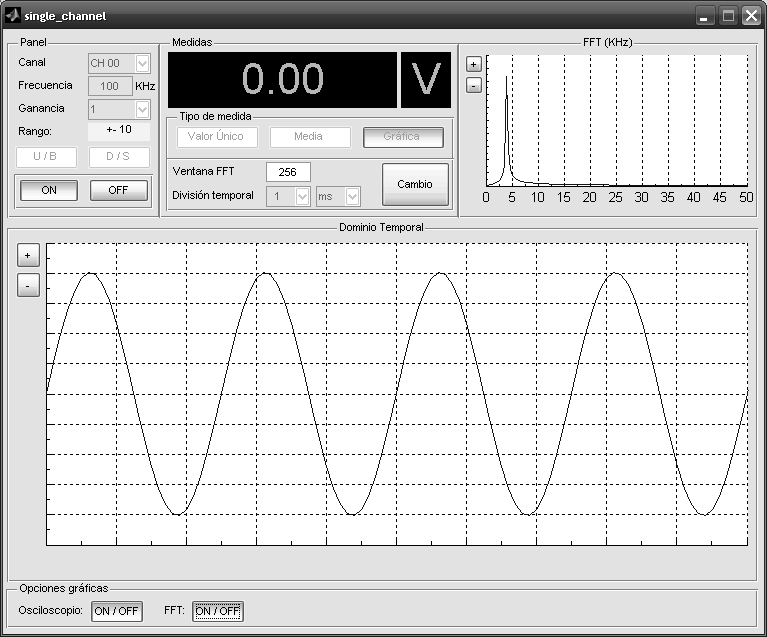
\includegraphics{gis-pfc-appa-01.png}
    \end{center}
    \caption[Aspecto de la interfaz de usuario]{Disposición de los
	distintos paneles de control y visualizadores en la interfaz de
	usuario.}
    \label{fig:interface}
\end{figure}

\begin{enumerate}
    \itembf{Panel de control principal} Alberga los controles que
	permiten configurar las propiedades básicas de la sesión de
	adquisición.
    \itembf{Panel de control secundario} Los mandos contenidos en
	este panel permiten controlar aspectos secundarios de la sesión de
	adquisición.
    \itembf{Visor} En el visor se muestran los resultados
	numéricos.
    \itembf{Ventana de representación grande} En esta ventana la
	representación ocupa un tamaño mayor.
    \itembf{Ventana de representación pequeña} En esta ventana la
	representación se hace a escala reducida.
    \itembf{Controles gráficos} Permiten habilitar o inhabilitar una o
	ambas representaciones gráficas.
\end{enumerate}


\subsection{Panel de control principal}

A continuación se enumeran los distintos botones y visualizadores que
integran el panel de control, su disposición en el panel se ilustra en la
\vref{fig:firstcontrolpanel}.

\begin{enumerate}
    \itembf{Selector de canal} Permite seleccionar el canal del que se
	extrae información. Sólo se puede seleccionar un canal a la vez.
    \itembf{Selector de frecuencia} Permite ajustar la frecuencia de
	muestreo de la tarjeta de adquisición. El valor de la frecuencia de
	muestreo debe estar contenido entre 1 kHz y la máxima frecuencia de
	muestreo permitida.
    \itembf{Control de ganancia} Ajusta la ganancia del amplificador de
	instrumentación integrado en la tarjeta. Determina el rango máximo
	de variación de la señal de entrada.
    \itembf{Indicador de rango} Rango máximo en el que debe estar contenida
	la señal de entrada (si la señal excede este rango tras ser
	amplificada internamente satura el conversor \sig{a/d} de la
	tarjeta de adquisición).
    \itembf{Control \sig{u/b}} Controla el modo de adquisición
	(unipolar/bipolar).
    \itembf{Control d/s} Controla el modo de terminación
	(diferencial/sencillo). Altera el comportamiento del selector de
	canal (lista 8 canales en modo diferencial y 16 en modo sencillo).
    \itembf{Control de on/off} Inicia o detiene respectivamente la sesión
	de adquisición.
\end{enumerate}


\subsection{Panel de control secundario}

Los elementos contenidos en el panel de control secundario son los listados
a continuación. La \cref{fig:secondcontrolpanel} muestra su ubicación
relativa en el panel.

\begin{enumerate}
    \itembf{Selector de tipo de medida} Permite seleccionar el tipo de
	resultado devuelto: muestra individual, media aritmética o
	representación gráfica de la señal y su espectro en frecuencia.
    \itembf{Ventana \sig{fft}} Permite seleccionar el número de puntos con
	el que se realiza la \sig{fft} utilizada para representar el
	espectro de la señal.
    \itembf{División temporal} Controla la duración del fragmento de señal
	representado gráficamente. Activa o desactiva el modo de
	representación continuo.
    \itembf{Cambio de ventana} Intercambia la ventana (ventanas de
	representación grande y pequeña) en la que se representan
	gráficamente la señal y su espectro en frecuencia.
\end{enumerate}

\newlength{\biggestpanel}
\settoheight{\biggestpanel}{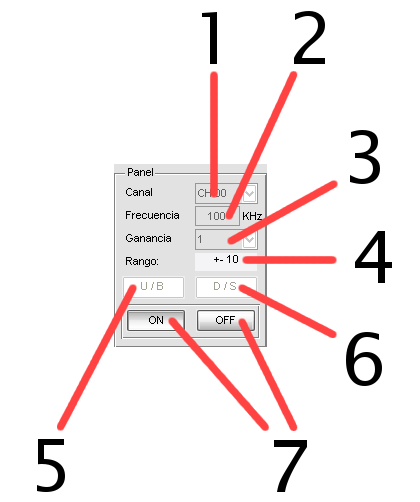
\includegraphics{gis-pfc-appa-02.png}}

\begin{figure}
    \begin{center}
	\subfloat[Elementos del panel de control principal][Panel de
	    control principal.]{
	    \label{fig:firstcontrolpanel}
	    \begin{minipage}[top][\biggestpanel][c]{.425\textwidth}
		\centering
		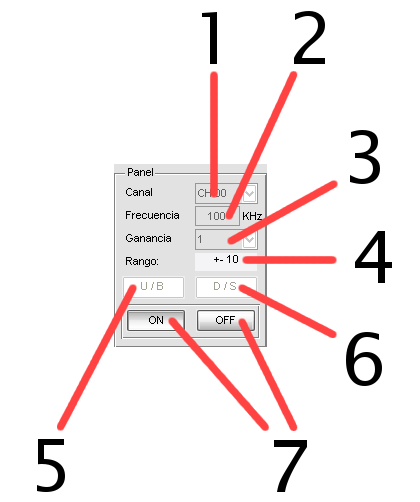
\includegraphics{gis-pfc-appa-02.png}
	    \end{minipage}}
	\subfloat[Elementos del panel de control secundario][Panel de
	    control secundario.]{ \label{fig:secondcontrolpanel}
	    \begin{minipage}[top][\biggestpanel][c]{.425\textwidth}
		\centering
		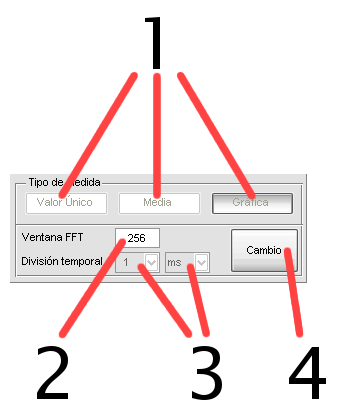
\includegraphics{gis-pfc-appa-03.png}
	    \end{minipage}}
    \end{center}
    \caption[Paneles de control de la interfaz de usuario]{Esta figura
    muestra los distintos elementos que integran los paneles de control
    principal y secundario de la interfaz de usuario.}
    \label{fig:controlpanels}
\end{figure}

\subsection{Visor}

En el visor se pueden observar los resultados que proporcionan los modos de
funcionamiento numéricos. Los resultados se dan con una precisión de
decenas de milivoltios.


\subsection{Ventanas de representación grande y
pequeña}\label{subsec:windows}

Las representaciones se realizan en estas dos ventanas, cada ventana
alberga simultáneamente una única representación. El control de cambio de
ventana permite intercambiar la ventana en la que se representan señal y
espectro en frecuencias, por defecto la señal se representa en la ventana
grande y su espectro frecuencial en la ventana pequeña. Al pulsar el botón
cambio de ventana se intercambian también las marcas de gráfico, el título
y la rejilla. Los controles situados en el margen de cada ventana duplican
o dividen por dos la escala de amplitud de la representación.

\subsection{Controles gráficos}\label{subsec:gfoptions}

Los controles de este panel gráfico habilitan o inhabilitan la
representación gráfica de la señal y de su espectro en frecuencia
respectivamente. No tienen ninguna función en los modos numéricos de
funcionamiento.


\section{Inicio y detención de la sesión de adquisición}

El control \func{on} del panel principal de la interfaz de usuario inicia
la sesión de adquisición. Por su parte el control \func{off} detiene el
muestreo. Al pulsar en el control \func{on} se inhabilitan todos los
controles de la interfaz de usuario exceptuando los siguientes: control
\func{off}, ventana \sig{fft}, cambio de ventana, controles de las ventanas
de representación y controles del panel opciones gráficas. Al pulsar
\func{off} todos los controles inhabilitados se restablecen.


\section{Modos de funcionamiento}

Existen tres modos de funcionamiento: muestra individual, media aritmética
y representación gráfica. Cada uno de ellos aporta distintos resultados.


\subsection{Muestra individual}

En este modo el visor muestra el valor de la última muestra adquirida (la
frecuencia de adquisición es de 4 Hz).

Si la señal evaluada oscila a una frecuencia elevada los valores observados
cambian rápidamente por lo que no resultan nada útiles.


\subsection{Media aritmética}

En este modo el visor muestra la media aritmética de las muestras
adquiridas en un espacio de tiempo de 250 ms. El número de muestras
utilizado para realizar la media depende de la frecuencia de muestreo (la
frecuencia de adquisición puede ajustarse mediante el selector de
frecuencia).

El visor se refresca cada 250 ms cuando este modo está activado. Si la
señal estudiada oscila rápidamente en el visor puede observarse el valor
<<$0.00$>>.


\subsection{Representación gráfica}

En este modo de funcionamiento se muestra el aspecto de la señal y el de su
espectro en frecuencias. Al seleccionar el modo de funcionamiento gráfico
se inhabilita el selector de frecuencia y se fija la frecuencia de muestreo
a la máxima frecuencia de muestreo posible (100 kHz si no se han añadido
más canales al objeto dispositivo asociado a la tarjeta).

Según la configuración del control división temporal (que determina la
duración del fragmento de señal representado por pantalla) se utiliza uno
de los dos modos de representación implementados.


\subsubsection{Modo de representación disparado}

La representación de la señal se muestra fija en el centro de la ventana de
representación. Este modo es útil para observar señales que oscilan a
frecuencias por encima de los 4 Hz, el disparo falla cuando se observan
señales que oscilan a una frecuencia inferior. Permite determinar
fácilmente la amplitud y la frecuencia de oscilación de la señal.


\subsubsection{Modo de representación continuo}

Este modo de representación se activa cuando la escala temporal de la
representación (control división temporal) se ajusta por encima de los 4
ms. En este modo la representación de la señal se desplaza de derecha a
izquierda a medida que avanza el tiempo. Este modo de representación es
útil para observar la forma de señales que oscilan a frecuencias inferiores
a los 4 Hz. También puede ayudar a determinar la amplitud de una señal. Sin
embargo es difícil averiguar la frecuencia a la que oscila una señal
observando la representación obtenida al activar este modo.


\section{Salida y limpieza}

Al cerrar la aplicación se detiene el proceso de muestreo y se elimina
último canal asignado al objeto dispositivo (si antes no se ha eliminado
ningún canal).

Al terminar la aplicación es necesario eliminar el objeto dispositivo y
limpiar el área de trabajo de \matlab{}.

\begin{center}
    \begin{lstlisting}
	aux = daqfind
	delete(aux);
	clear aux;
    \end{lstlisting}
\end{center}
